\documentclass[10pt,letterpaper]{article}
\usepackage{geometry}
\geometry{margin=1in}
\usepackage{graphicx}
 \usepackage{amsmath} 
\usepackage{tikz}
\usepackage{xcolor}
\usepackage{pdflscape}
\usepackage{booktabs}
\usepackage{cite}
\usepackage[sorting=none]{biblatex}
\addbibresource{reference.bib}

\usetikzlibrary{arrows,shapes,positioning,fit,backgrounds}

\setlength{\parindent}{0pt}
\setlength{\parskip}{0.5em}

%make lists tighter
\usepackage{enumitem}
\setlist{nolistsep}

%reduce spacing before and after section
\usepackage{titlesec}
% reduce section, subsection, etc spacing
\usepackage{titlesec}
\titlespacing*{\section}{0pt}{0\baselineskip}{0\baselineskip}
\titlespacing*{\subsection}{0pt}{0\baselineskip}{0\baselineskip}
\titlespacing*{\subsubsection}{0pt}{0\baselineskip}{0\baselineskip}

%reduce list spacing
\usepackage{enumitem}
\setlist{nosep}

\usepackage[hidelinks]{hyperref}

\title{Lab 2 - Cloud Data, Stat 214, Spring 2025\vspace{-2em}}

% submission must not contain any of your names
% but feel free to make a version for yourself with your names on it
% \author{Your names}

\begin{document}
\maketitle


\section{Introduction}
As global temperatures rise and carbon dioxide levels increase, accurate cloud detection has become a critical challenge, particularly in the Arctic. The difficulty arises from the optical similarity between ice-covered surfaces and clouds, making traditional methods based on color and temperature ineffective. In their paper \textit{"Daytime Arctic Cloud Detection Based on Multi-Angle Satellite Data With Case Studies"} Tao Shi et al. \cite{shi2008} systematically investigate Arctic cloud detection and propose two new algorithms. The first, Enhanced Linear Correlation Matching (ELCM), identifies cloud-free surface pixels using features such as CORR, SDAn, and NDAI. The second method builds on ELCM by incorporating Quadratic Discriminant Analysis (QDA) to refine classification results.

In our work, we extend this research on Arctic cloud detection using  Multi-angle Imaging SpectroRadiometer (MISR) satellite images, a dataset designed for analyzing cloud cover in polar regions, which provides additional perspective that help distinguish clouds from similar-looking surface, such as ice and snow. Our goal is to develop a more effective algorithm for distinguishing clouds from non-clouds surfaces. Our study begins with Exploratory Data Analysis (EDA) to visualize cloud and non-cloud pixels, compare the distributions of key features in two pixels, and explore the interdependence between features using correlation heatmap. Next, we conduct data processing, including cleaning missing or invalid values and normalizing numerical features to ensure consistency across the dataset. To improve classification performance, we implement autoencoders to find the most effective embeddings for classification. For the modeling part, we use both 8-dimensional and 16-dimensional embeddings to train multiple classifiers and evaluate model performance using cross-validation, ROC AUC, and feature importance analysis. Finally, we analyze misclassifications to identify patterns in errors and assess the trade-offs between different modelings. 


\section{EDA}

\subsection{Images Visualization}

In the Figure 1, we colored points based on the cloud presence, with blue representing clouds, red representing no clouds, and grey representing unlabeled data. 

\begin{figure}[h!]
    \centering
    \includegraphics[width=\textwidth]{pics/cloud.png}  
    \label{fig:cloudmap}
    \caption{Cloud map}
\end{figure}

\subsection{Exploring Relationships among Features}

We explored how different features, such as NDAI, SD, and CORR, relate to cloud presence. To identify potential patterns or differences between the two classes, we visualized these relationships by plotting histograms of each feature for both cloud and non-cloud classes. 

The given plots show the distributions of various features (NDAI, SD, CORR, and different radiance values) for cloud and non-cloud pixels. The key observations from each plot are:

1) NDAI (Normalized Difference Angular Index) differs significantly between cloud and non-cloud pixels. It appears to have a strong peak around 0.05–0.2, where most non-cloud pixels (red) are concentrated. In contrast, cloud pixels (blue) have a wider and spread, with more values spanning approximately 0.1 to 0.8. However, there is some overlap between the two distributions, particularly in the low NDAI range from 0.05 to 0.2, which may cause some challenge in classification. Despite this, the difference in patterns suggests that NDAI might be useful in distinguishing clouds from non-clouds, as clouds generally tend to have higher NDAI values.

2) SD (Standard Deviation of Local Image Intensity) shows a heavy skew towards lower values, with most pixels having SD close to zero.  Non-cloud pixels (red) dominate at very low SD values. Cloud pixels (blue) have a broader range of SD values, suggesting more variability in local intensity. The large difference in distributions indicates that SD could be a valuable feature for classification, since the cloud pixels are likely to have higher SD values.

3) CORR (Correlation of Local Image Patches) exhibits a strong concentration near 1.0 for both classes, meaning that image patches tend to be highly correlated. Non-cloud pixels (red) appear more concentrated at the highest correlation values, while cloud pixels (blue) have a slightly more spread-out distribution. This implies that non-cloud pixels may be more homogeneous in texture, whereas cloud pixels show more variation.

4) Radiance DF: Non-cloud pixels (red) tend to cluster around 25,000–30,000 with a high peak, indicating that their radiance values are relatively concentrated. In contrast, cloud pixels (blue) show a boarder and more dispersed distribution, implying greater variability in their radiance levels. The distinction in their concerntration patterns suggests that Radiance DF could be useful in cloud classification.

5) Radiance CF: A similar trend is observed in this feature, where non-cloud pixels (red) again form distinct peaks around 20,000–30,000, suggesting that non-cloud regions tend to have characteristic brightness levels. The cloud pixels (blue) display a wider spread, indicating higher variability in radiance levels. This radiance feature can also contribute to differentiating cloud from non-cloud pixels, as the greater dispersion in cloud radiance shows that clouds could have more optical properties which are influenced by various factors.

6) Radiance BF: Similar trends as the previous radiance plots: non-cloud pixels (red) have sharp peaks, while cloud pixels (blue) are more spread out. Some overlap is present, but the differences in peak intensity could aid classification.

Overall, SD and NDAI appear to be the most distinctive features, with clear differences between cloud and non-cloud pixels. Radiance values (DF, CF, BF) show significant differences in peak intensity, which suggests they could help separate the classes. CORR is less separable, but cloud pixels tend to cluster more at high correlation values.

\begin{figure}[htbp]
    \centering
    \includegraphics[width=0.85\textwidth]{pics/plot2.png}  
    \caption{Distribution by Variable}
    \label{fig:plot2}
\end{figure}

\subsection{Data Splitting}

We divided the data set into training (60\%), validation (20\%) and test (20\%) sets. The decision to allocate 60\% of the data to the training set is based on the need for the model to learn from a sufficiently large portion of the data. A larger training set allows the model to better understand the underlying patterns and features associated with cloud and non-cloud pixels.

The 20\% allocated to the validation set is used to tune the model's hyperparameters and assess its performance during the training process. This set is crucial for preventing overfitting by making sure that the model does not simply memorize the training data, but learns to generalize effectively to unseen data. The validation set helps identify the optimal configuration of the model before the final evaluation of the test set.

The remaining 20\% of the data is reserved for the test set, which provides an unbiased evaluation of the model's performance after training and validation. This set ensures that the final evaluation reflects the model’s ability to perform on data it has never seen before, which is critical for assessing how well the cloud detection algorithm would perform in real-world scenarios, where it will be applied to new satellite images.

The split (train set: 124,609 samples, validation set: 41,536 samples, test set: 41,536 samples) ensures a balanced distribution of data, providing enough samples for each set to contribute meaningfully to the training, validation, and testing phases of model development. We will do the random splitting first. \textbf{Moreover, we will discuss the leave-one-image-out method in the modeling section. It helps prevent potential data leakage, since if our training set contains data from all three images, we are likely to leak some information to the model, as the pixels are not independent.} Therefore, it is necessary to keep one image untouched to ensure that our models generalize well to unseen data.

\subsection{Data Cleaning}

In this section, we performed comprehensive data cleaning and preprocessing to ensure high-quality input for cloud detection analysis. Below are the key steps taken:

1) Handling Missing Values and Duplicates

First, we checked for missing values in each column and removed any rows containing missing data. Additionally, duplicate rows were identified and removed to prevent redundancy. This step ensures that the dataset is free of inconsistencies that may negatively impact model performance.

2) Removing Negative Radiance Values

Satellite radiance values are expected to be non-negative. Therefore, we scanned the dataset for negative values in the radiance-related columns (Radiance DF, Radiance CF, Radiance BF, Radiance AF, Radiance AN). Any rows containing negative values in these columns were removed to maintain data integrity.

3) Filtering Labeled Pixels

The dataset contained pixels that were either labeled as cloud/no-cloud or left unlabeled. To ensure that only meaningful data points are analyzed, we removed rows where the Label column had a value of 0 (unlabeled pixels). This step helps avoid unnecessary noise in the dataset.

4) Feature Normalization

After cleaning the dataset, we standardized the numerical features to ensure the consistency in scale. The selected features—Radiance DF, Radiance CF, Radiance BF, Radiance AF, Radiance AN, NDAI, SD, and CORR—were transformed to have a mean of zero and a standard deviation of one. This normalization ensures that all features contribute equally to model training, preventing dominance by larger numerical values and improving the overall stability of the model. 


\section{Feature Engineering}

\subsection{Identifying Three Most Important Features}

Before finding out the most important feature for distinguishing the labels, we would like to find out whether there exists any internal correlation among the 8 features we have. By understanding these relationships, we can identify the possible multicollinearity and avoid redundancy by selecting a diverse set of features or combining some features. Therefore, we plot a heatmap for both non-cloud and cloud pixels to visualize the inner dependencies among the features and investigate how the relationships vary for the two labels.

\begin{figure}[htbp]
    \centering
    \includegraphics[width=1.0\textwidth]{pics/Heatmap2.1.png}  
    \caption{Heatmap for Current 8 Features}
    \label{fig:heatmap2.1}
\end{figure}

From Figure \ref{fig:heatmap2.1}, we observe that the five radiance-related features are highly correlated within both non-cloud and cloud pixels, as seen in the top left corner of the plots. This suggests that these five features may carry redundant information. Moreover, we find that the correlation of SD and NDAI with the five radiance-related features differs between non-cloud and cloud pixels. For instance, the average correlation of SD with the five radiance features is approximately -0.65 for non-cloud pixels, whereas it remains around -0.25 for cloud pixels. However, the average correlation of NDAI with the radiance features is -0.75 for cloud pixels, but only -0.45 for non-cloud pixels. These results indicate that NDAI shows a stronger correlation with radiance features in cloud pixels, while SD exhibits a higher correlation with  radiance features in non-cloud pixels. The two heatmaps give us a rough idea of the importance of each feature.

To further investigate which feature is the most important, we need a method to quantify how much each pixel contributes to the label. One way to measure this relationship is by evaluating the correlation between features and the label. For this question, we will apply the Pearson Correlation, which reflects the linear relationship between the outcome and the independent variables. Usually, the value of the Pearson Correlation is between -1 to 1, so we can measure the importance of each feature by comparing the absolute value of its Pearson Correlation.

\begin{figure}[htbp]
    \centering
    \includegraphics[width=0.8\textwidth]{pics/PearsonCorr.png}  
    \caption{Pearson Correlation with Cloud Label}
    \label{fig:pearson}
\end{figure}

From Figure \ref{fig:pearson}, we have ranked the features with their absolute value of Pearson Correlation. The three most important features are NDAI, SD, and Radiance AF with values of 0.568, 0.495, and $-0.491$ respectively. Also, we have applied a random forest classifier in our code. The result reflects that the NDAI, SD, and Radiance AN are the three most important features while Radiance AF is the fourth important feature. Combining the two metrics, we can justify that NDAI, SD, and Radiance AF are the three most important features.

\subsection{Creating New Features}

One of the most intriguing parts is to construct our own features in machine learning. Before we create any new features, we have to think carefully about the inner structure of our data. Since the data is pixels within three images, we have to consider the patches instead of separate pixels as it can reconstruct the information \cite{lin2013patch} (Lin et al., 2013). Therefore, the following three features are the identity of a 9x9 patch which is centered at a certain pixel. 

The first feature is called patch range, which counts for the range of all the pixels as we would expect a smaller range if all the pixels in the patch share the same label. It is the first attempt for us to investigate some patterns within the patches. Moreover, we invented the gradient mean to measure the speed of transition within a certain patch, where a higher gradient mean may suggest the edges between cloud and non-cloud. The last feature is the variance explained by the first principle component. This feature is inspired by the idea that PCA is an excellent method for compressing the data in analyzing cloud images \cite{venkatakrishnamoorthy2019cloud} (Venkatakrishnamoorthy \& Reddy, 2019) . We expected that a smaller value of the PCA-explained variance would lead to a higher probability that the patch belongs to a more homogeneous region and the pixels are similar to each other. In conclusion, by introducing these three features, we would like to capture different aspects of pixel distribution and transitions within a patch. Thus, the patch range provides an overall measure of pixel variation, while gradient mean reflects edge-like structures where cloud transitions occur, and PCA-explained variance measures the dominant pattern within a patch.


\begin{figure}[htbp]
    \centering
    \includegraphics[width=1.0\textwidth]{Label_Heat.png}
    \caption{Expert Labels v.s. Mean Gradient Heatmap}
    \label{fig:label_heat}
\end{figure}

From Figure \ref{fig:label_heat}, we can observe that the gradient mean performs well in distinguishing cloud from non-cloud pixels. When we painted values above the average in red, we can find out that the image is similar to the original one. However, misclassifications still occur in certain corner cases especially when X is close to 0. Furthermore, the Pearson correlation coefficients are 0.577, $-0.668$, and 0.511 for gradient mean, PCA-explained variance, and patch range, respectively. Overall, all three features show meaningful associations with the labels and are suitable for further analysis at this stage.


\subsection{Autoencoder}

\begin{figure}[h]
\centering
\begin{minipage}{0.5\textwidth}
    \centering
    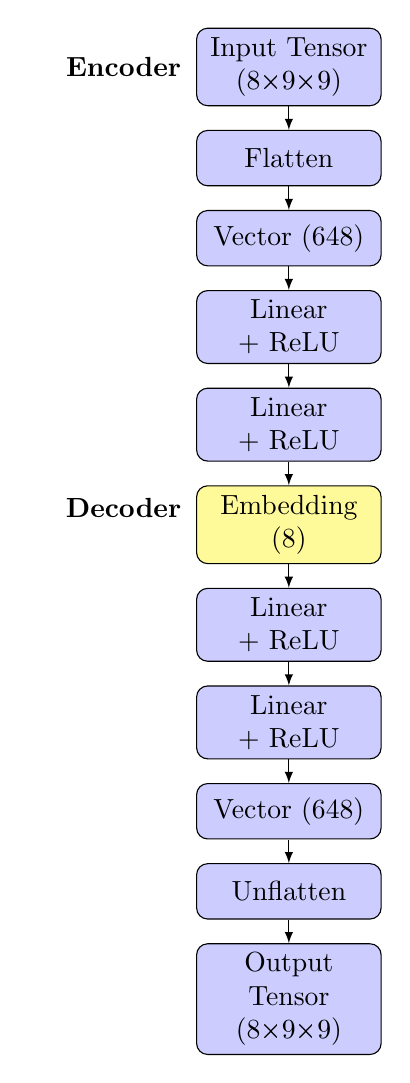
\begin{tikzpicture}[
        block/.style={rectangle, draw, fill=blue!20, 
                      text width=6em, text centered, rounded corners, minimum height=2em},
        line/.style={draw, -latex},
        scale=0.7  % Scale down to fit side by side
    ]
    \node [block] (input) {Input Tensor\\(8×9×9)};
    \node [block, below=0.3cm of input] (flatten1) {Flatten};
    \node [block, below=0.3cm of flatten1] (vec1) {Vector (648)};
    \node [block, below=0.3cm of vec1] (fc1) {Linear + ReLU};
    \node [block, below=0.3cm of fc1] (fc2) {Linear + ReLU};
    \node [block, below=0.3cm of fc2, fill=yellow!40] (emb) {Embedding (8)};
    \node [block, below=0.3cm of emb] (fc3) {Linear + ReLU};
    \node [block, below=0.3cm of fc3] (fc4) {Linear + ReLU};
    \node [block, below=0.3cm of fc4] (vec2) {Vector (648)};
    \node [block, below=0.3cm of vec2] (unflatten) {Unflatten};
    \node [block, below=0.3cm of unflatten] (output) {Output Tensor\\(8×9×9)};

    \draw [line] (input) -- (flatten1);
    \draw [line] (flatten1) -- (vec1);
    \draw [line] (vec1) -- (fc1);
    \draw [line] (fc1) -- (fc2);
    \draw [line] (fc2) -- (emb);
    \draw [line] (emb) -- (fc3);
    \draw [line] (fc3) -- (fc4);
    \draw [line] (fc4) -- (vec2);
    \draw [line] (vec2) -- (unflatten);
    \draw [line] (unflatten) -- (output);

    % Labels
    \node[text width=2.2cm, text centered] at (-3,0) {\textbf{Encoder}};
    \node[text width=2.2cm, text centered] at (-3,-8) {\textbf{Decoder}};
    \end{tikzpicture}
    \caption{Baseline Architecture}
    \label{fig:baseline}
\end{minipage}%
\hfill
\begin{minipage}{0.5\textwidth}
    \centering
    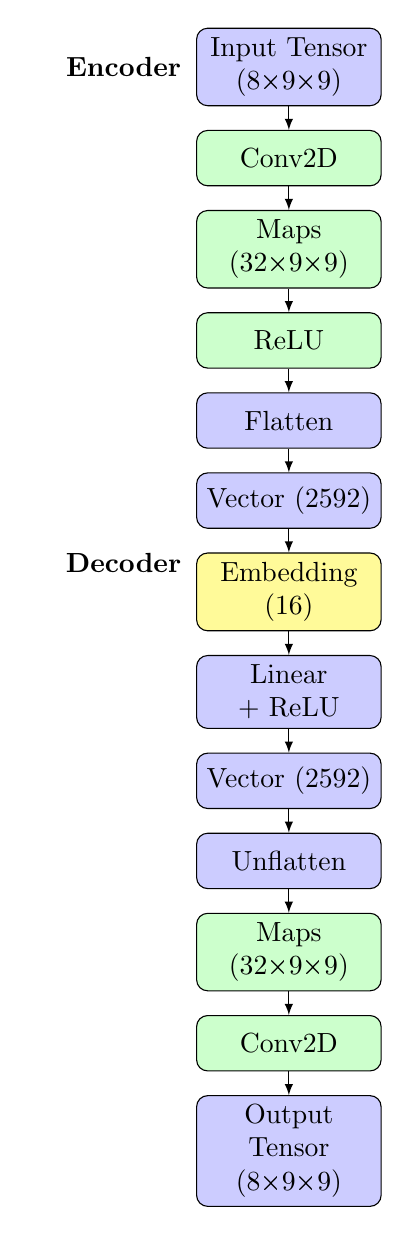
\begin{tikzpicture}[
        block/.style={rectangle, draw, fill=blue!20, 
                      text width=6em, text centered, rounded corners, minimum height=2em},
        convblock/.style={rectangle, draw, fill=green!20, 
                      text width=6em, text centered, rounded corners, minimum height=2em},
        line/.style={draw, -latex},
        scale=0.7  % Scale down to fit side by side
    ]
    \node [block] (input) {Input Tensor\\(8×9×9)};
    \node [convblock, below=0.3cm of input] (conv1) {Conv2D};
    \node [convblock, below=0.3cm of conv1] (feat1) {Maps (32×9×9)};
    \node [convblock, below=0.3cm of feat1] (relu1) {ReLU};
    \node [block, below=0.3cm of relu1] (flatten) {Flatten};
    \node [block, below=0.3cm of flatten] (vec1) {Vector (2592)};
    \node [block, below=0.3cm of vec1, fill=yellow!40] (emb) {Embedding (16)};
    \node [block, below=0.3cm of emb] (linear) {Linear + ReLU};
    \node [block, below=0.3cm of linear] (vec2) {Vector (2592)};
    \node [block, below=0.3cm of vec2] (unflatten) {Unflatten};
    \node [convblock, below=0.3cm of unflatten] (feat2) {Maps (32×9×9)};
    \node [convblock, below=0.3cm of feat2] (conv2) {Conv2D};
    \node [block, below=0.3cm of conv2] (output) {Output Tensor\\(8×9×9)};

    \draw [line] (input) -- (conv1);
    \draw [line] (conv1) -- (feat1);
    \draw [line] (feat1) -- (relu1);
    \draw [line] (relu1) -- (flatten);
    \draw [line] (flatten) -- (vec1);
    \draw [line] (vec1) -- (emb);
    \draw [line] (emb) -- (linear);
    \draw [line] (linear) -- (vec2);
    \draw [line] (vec2) -- (unflatten);
    \draw [line] (unflatten) -- (feat2);
    \draw [line] (feat2) -- (conv2);
    \draw [line] (conv2) -- (output);

    % Labels
    \node[text width=2.2cm, text centered] at (-3,0) {\textbf{Encoder}};
    \node[text width=2.2cm, text centered] at (-3,-9) {\textbf{Decoder}};
    \end{tikzpicture}
    \caption{Simplified Architecture}
    \label{fig:simplified}
\end{minipage}
\end{figure}


In this study, we explored various autoencoder architectures to learn meaningful representations from MISR data that can better distinguish between clouds and polar surfaces.

Autoencoders are neural networks designed to learn efficient encodings of input data by attempting to reconstruct the original input from a compressed representation. By forcing the network to pass information through a bottleneck (the embedding layer), autoencoders learn to preserve the most salient features of the data. In our context, we hypothesize that different architectural choices will impact the quality of these learned representations and subsequently affect cloud detection performance.

For our autoencoder experiments, we employed a consistent configuration across all architectures to ensure
fair comparison. The key hyperparameters were as follows

\begin{itemize}
    \item Patch Size: 9×9 pixels around each point, capturing local context
    \item Input Channels: 8 channels including NDAI, SD, CORR, and the five radiance measurements
    \item Batch Size: 2048 for both training and validation
    \item  Learning Rate: 0.001 using Adam optimizer
    \item Maximum Epochs: 50 with early stopping based on validation loss
    \item Workers: 4 parallel data-loading processes for efficient training
    \item Embedding Size: 16-dimensional encoding space and 8-dimensional encoding space
    \item Activation Functions: Varied by architecture (ReLU, GELU, or Swish)
    \item Logging Frequency: Training metrics recorded every 50 steps
    \item Validation: Performed after each epoch on 20\% of data
\end{itemize}


We implemented and evaluated four different autoencoder architectures: a baseline model, a simplified architecture, a deep architecture with GELU activation, and a residual architecture with Swish activation. Each architecture represents different trade-offs in terms of model complexity, training efficiency, and representational capacity. 

The MISR dataset consists of 164 satellite images, with only 3 containing expert labels for cloud presence. Each image contains approximately 115,378 pixels, with each pixel represented by a 9×9 patch across 8 different channels: NDAI, SD, CORR, and five radiance measurements at different viewing angles (DF, CF, BF, AF, AN).
For our autoencoder training, we use 161 unlabeled images and extract 9×9 patches centered around each pixel, resulting in input tensors of shape (8, 9, 9). The large number of unlabeled images allows us to leverage unsupervised pre-training, following a transfer learning approach where we first train the autoencoder on all images without using labels, then use the learned embeddings to train a supervised classifier on the labeled subset. \textbf{To prevent data leakage, we train the autoencoder model using 80\% of the total 161 unlabeled images, rather than randomly selecting 80\% of the 9×9 patches from all images.} This approach makes sure that training and validation patches are derived from distinct images. In general, it preserves the integrity of the evaluation process and prevents information from leaking across the training and validation sets. The model was optimized to minimize the loss function during training.

\subsubsection{Baseline Architecture}

Followed by \ref{fig:baseline}, baseline architecture follows a traditional fully-connected autoencoder design. This architecture flattens the 3D input tensor into a 1D vector, progressively reducing the dimension through fully-connected layers until reaching the embedding size of 8. The decoder mirrors this structure to reconstruct the original input. While simple and computationally efficient, this approach discards the spatial relationships between pixels in each patch.
The baseline model contains approximately 184000 trainable parameters and uses ReLU activation functions throughout. Training is performed using the Adam optimizer with a learning rate of 0.001 and MSE loss for reconstruction.

\subsubsection{Simplified Architecture}

We add convolution layer and reduce model complexity by minimizing the number of layers and parameters. This architecture uses a single convolutional layer followed by a single fully-connected layer in the encoder, with a symmetric structure in the decoder. By incorporating a convolutional layer, it preserves some spatial information while still maintaining a minimal parameter count. With approximately 85000 parameters, this architecture trains faster and requires fewer computational resources than the baseline.

The trade-off is potentially reduced model capacity, which may limit the network's ability to learn complex patterns in the data. The simplified architecture is ideal for situations where computational resources are limited or when the underlying patterns are relatively simple.

\subsubsection{Deep Architecture with GELU Activation}
The deep architecture significantly increases model expressivity through additional layers and more sophisticated activation functions. This architecture introduces several key improvements:

\begin{itemize}
\item Multiple convolutional layers with increasing then decreasing channel dimensions (8 $\to$ 32 $\to$ 64 $\to$ 128 $\to$ 64), creating a hierarchical feature extraction pattern
\item Batch normalization after each convolutional layer to stabilize training and improve convergence
\item GELU activation (Gaussian Error Linear Unit), which provides smoother gradients than ReLU
\item Deeper fully-connected layers in the bottleneck, allowing more complex transformations
\end{itemize}

The GELU activation function is defined as:
$\text{GELU}(x) = x \cdot \Phi(x)$ where $\Phi(x)$ is the cumulative distribution function of the standard normal distribution. GELU combines the benefits of ReLU with smoother gradients, which can help with optimization.

With approximately 3.2 million parameters, this is the most complex architecture among those tested. The increased capacity allows the model to learn more nuanced representations, potentially capturing subtle differences between clouds and ice surfaces that simpler models might miss.


\subsubsection{Residual Architecture with Swish Activation}

The residual architecture incorporates skip connections to improve gradient flow during training. 

This architecture introduces several innovations:

\begin{itemize}
    \item Residual connections (e2 = self.encoderconv2(e1) + e1), which allow gradients to flow directly through the network, mitigating the vanishing gradient problem
    \item Swish activation $(x * sigmoid(x))$, a self-gated activation function that has shown promising results in deep networks
    \item Component-wise implementation rather than Sequential modules, allowing for more flexible connections between layers
    \item Dropout regularization (p=0.3) in the fully-connected layers to prevent overfitting
\end{itemize}

Residual connections are particularly valuable in deeper networks, as they create shortcuts that help gradients propagate during backpropagation. This can lead to more stable training and allows for successfully training deeper networks. Moreover, the Swish activation function combines the benefits of ReLU (not saturating for positive values) with smoother behavior near zero, potentially leading to better gradient flow during training.

\begin{figure}[h]
\centering
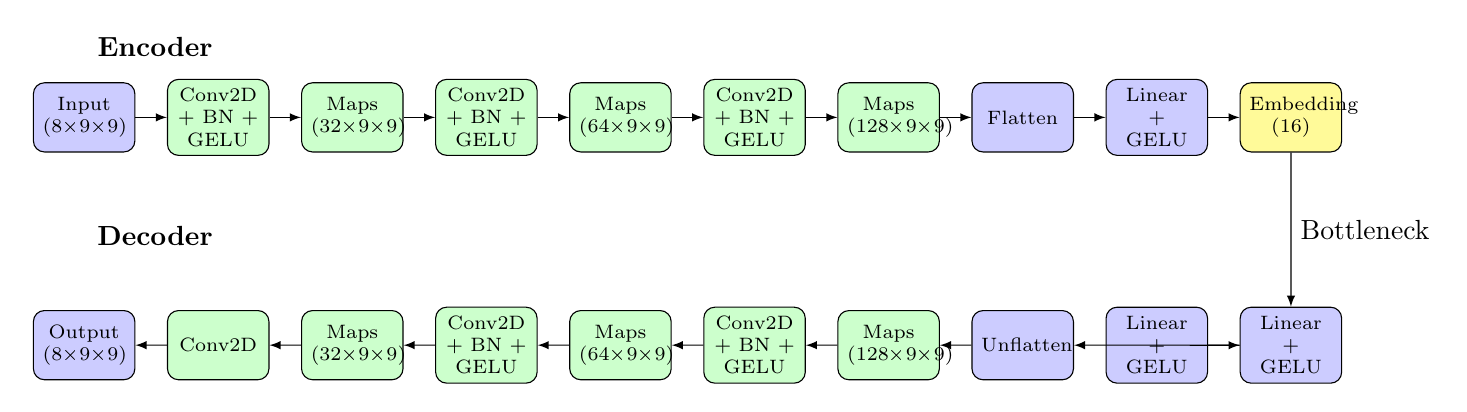
\begin{tikzpicture}[
    block/.style={rectangle, draw, fill=blue!20, 
                  text width=3em, text centered, rounded corners, minimum height=2.5em,  font=\scriptsize},
    convblock/.style={rectangle, draw, fill=green!20, 
                  text width=3em, text centered, rounded corners, minimum height=2.5em,  font=\scriptsize},
    line/.style={draw, -latex},
    scale=0.3  % Adjust scale as needed
]
% Encoder Section
\node [block] (input) {Input\\(8×9×9)};
\node [convblock, right=0.4cm of input] (conv1) {Conv2D + BN + GELU};
\node [convblock, right=0.4cm of conv1] (feat1) {Maps\\(32×9×9)};
\node [convblock, right=0.4cm of feat1] (conv2) {Conv2D + BN + GELU};
\node [convblock, right=0.4cm of conv2] (feat2) {Maps\\(64×9×9)};
\node [convblock, right=0.4cm of feat2] (conv3) {Conv2D + BN + GELU};
\node [convblock, right=0.4cm of conv3] (feat3) {Maps\\(128×9×9)};
\node [block, right=0.4cm of feat3] (flatten) {Flatten};
\node [block, right=0.4cm of flatten] (fc1) {Linear + GELU};
\node [block, right=0.4cm of fc1, fill=yellow!40] (emb) {Embedding\\(16)};

% Decoder Section (on a new line below)
\node [block, below=2cm of input] (output) {Output\\(8×9×9)};
\node [convblock, right=0.4cm of output] (conv8) {Conv2D};
\node [convblock, right=0.4cm of conv8] (feat8) {Maps\\(32×9×9)};
\node [convblock, right=0.4cm of feat8] (conv7) {Conv2D + BN + GELU};
\node [convblock, right=0.4cm of conv7] (feat7) {Maps\\(64×9×9)};
\node [convblock, right=0.4cm of feat7] (conv6) {Conv2D + BN + GELU};
\node [convblock, right=0.4cm of conv6] (feat6) {Maps\\(128×9×9)};
\node [block, right=0.4cm of feat6] (unflatten) {Unflatten};
\node [block, right=0.4cm of unflatten] (fc2) {Linear + GELU};
\node [block, right=0.4cm of fc2] (fc3) {Linear + GELU};

% Connect encoder
\draw [line] (input) -- (conv1);
\draw [line] (conv1) -- (feat1);
\draw [line] (feat1) -- (conv2);
\draw [line] (conv2) -- (feat2);
\draw [line] (feat2) -- (conv3);
\draw [line] (conv3) -- (feat3);
\draw [line] (feat3) -- (flatten);
\draw [line] (flatten) -- (fc1);
\draw [line] (fc1) -- (emb);

% Connect decoder
\draw [line] (fc3) -- (unflatten);
\draw [line] (unflatten) -- (feat6);
\draw [line] (feat6) -- (conv6);
\draw [line] (conv6) -- (feat7);
\draw [line] (feat7) -- (conv7);
\draw [line] (conv7) -- (feat8);
\draw [line] (feat8) -- (conv8);
\draw [line] (conv8) -- (output);
\draw [line] (emb) -- node[right] {Bottleneck} (fc3);
\draw [line] (fc2) -- (fc3);

% Add encoder and decoder labels
\node[text width=3cm, text centered] at (3,3) {\textbf{Encoder}};
\node[text width=3cm, text centered] at (3,-5) {\textbf{Decoder}};

\end{tikzpicture}
\caption{Deep architecture with GELU activation functions and batch normalization, shown in a horizontal layout. The encoder (top) compresses information through multiple convolutional layers into a 16-dimensional embedding, while the decoder (bottom) reconstructs the original input.}
\label{fig:deep}
\end{figure}



\begin{figure}[htbp]
    \centering
    \begin{minipage}{0.48\textwidth}
    \includegraphics[width=1.0\textwidth]{pics/train_loss.png}  
    \caption{Autoencoder Training Loss}
    \label{fig:trainloss}
    \end{minipage}
    \hfill
    \begin{minipage}{0.48\textwidth}
    \includegraphics[width=1.0\textwidth]{pics/val_loss.png}  
    \caption{Autoencoder Validation Loss}
    \label{fig:valloss}
    \end{minipage}
\end{figure}


It can be shown that Deep Architecture with GELU activation performed best on the validation set. Its loss is around 0.06, outperforming other 3 models. Also, there is no evidence that the model is overfitting by looking at the training loss. The Residual Architecture is expected to get the lowest loss on validation set since it adds residual connection to avoid vanishing gradient and dropout regularization to avoid overfitting. However, it performs even worse than simple architecture which only uses 1 convolutional layer. 

Now, we use the embeddings from this best-performing Deep Architecture for downstream classification task. This gives us the embedding of 16-dimensional space for each pixel in labeled picture. 


\section{Modeling}

Using the selected features, we developed four binary classifiers for prediction, including logistic regression, decision tree, neural network, and XGBoost. We proposed two approaches to modeling. First, we use the deep architecture shown above but we only use 8-dimensional embedding and 16-dimensional embedding. 

Table \ref{tab:classification_counts} presents the distribution of cloud and non-cloud pixels across the three labeled images. The dataset does not exhibit a significant class imbalance, allowing us to use accuracy or F1-score as appropriate evaluation metrics for classification performance.

\begin{table}[h]
    \centering
    \begin{tabular}{lc}
        \toprule
        Label    & Count  \\
        \midrule
        Not-Cloud  & 126716 \\
        Cloud      & 80965  \\
        \bottomrule
    \end{tabular}
    \caption{Classification Counts}
    \label{tab:classification_counts}
\end{table}

\subsection{8-dimensional embedding}

\subsubsection{Logistic Regression}

Before we apply the logistic regression model, we first have to check whether there exists multicollinearity in the features. Although the data we have here are extracted from three plots, which suggested the underlying correlation, we can still calculate the variance inflation factor (VIF) to find out potential redundant features. We assessed the Variance Inflation Factor (VIF) for each variable and removed those with VIF scores greater than 10, which is a judgment call made by us to determine whether a feature should be modified or not.

Our analysis identified “grad\_mean” and “patch\_range” as variables with high VIF scores since both of them measure the sparsity of the image. To reduce redundancy while preserving information, we combined these variables into one feature by Principal Component Analysis (PCA). 

After addressing the multicollinearity problem, the data satisfied the assumption for the logistic regression model. To prepare for model training, we split the dataset into 60\% training, 20\% validation, and 20\% test sets (another approach in the next section). Model evaluation is conducted using Accuracy, which quantifies the proportion of correctly classified instances, and ROC AUC, which assesses the model’s ability to  successfully distinguish between the classes. Also, to enhance the robustness of our performance estimates, we performed a 10-fold stratified cross-validation. By this way, we can ensure that class distribution is maintained across training and validation folds.

The overall model shows strong predictive performance, with an accuracy of 0.946 and ROC AUC of 0.976. This indicates that the model correctly classifies 94.6\% of the data, and shows an outstanding performance in distinguishing between the two classes. Additionally, it has an AIC of 45911.73. 

\begin{table}[h]
    \centering
    \begin{tabular}{lc}  
        \toprule
        \textbf{Features} & \textbf{Odd Ratio}\\
        \midrule
        ae5 & 10.055 \\  
        ae0 & 3.588  \\ 
        ae4 & 2.692   \\
        ae1 & 2.111  \\
        CORR & 1.468 \\ 
        \bottomrule
    \end{tabular}
    \caption{Top 5 Features with the Highest Odds Ratios}
    \label{tab:Odd Ratios}
\end{table}

According to the feature importance, pca\_feature turns out to be the most important feature in the model with a mean importance of 0.133, followed closely by ae5, which has a mean importance of 0.098. These results highlight the substantial contribution of these features to the model’s predictive accuracy.

As shown in Table \ref{tab:Odd Ratios}, we can analyze the odds ratio. For instance, ae5 has an odds ratio of 10.056, indicating that a one-unit increase in ae5 is associated with a 905.6\% increase in the odds of a positive outcome. Among the features of interest, CORR has an odds ratio of 1.468, meaning that each unit increase in CORR corresponds to a 46.8\% increase in the odds. Similarly, SD has an odds ratio of 1.246, implying a 24.6\% increase in the odds per unit increase in SD. Conversely, pca\_feature has the lowest odds ratio of 0.17, which means a one-unit increase in this feature results in an 83\% decrease in the odds of the positive class, suggesting that higher values of pca\_feature are associated with a reduced likelihood of the positive class.

Overall, the Logistic Regression model we constructed is simple but effective, as it achieves a 94.6\% accuracy and a ROC score of 0.976, which is a remarkable result compared to the ELCM algorithm that Shi et al. \cite{shi2008} proposed in their paper. As the first model, it sets up a strong starting point for our further research. Moreover, the coefficients are easy to interpret, as they are directly linked to the odds ratios after exponential transformation.

\subsubsection{Decision Tree}

Next, we built a decision tree classifier to further evaluate the predictive power of the selected features. Decision trees operate by recursively splitting the data into subsets based on input features, with each split forming two distinct groups. They are particularly advantageous due to their ability to capture nonlinear relationships within the data while maintaining high interpretability, making them a powerful tool for feature evaluation and predictive modeling. To optimize the model’s performance, we conducted hyperparameter tuning using GridSearchCV, testing various values for maximum depth, minimum sample perleaf, and minimum samples per split. 

The hyperparameter tuning process determined that a maximum depth of 10, minimum sample leaf of 5, and minimum sample split of 5 generates the best result. The model trained with these hyperparameters achieved the ROC AUC score of 0.989, indicating an excellent ability to distinguish between two classes. Additionally, when tested on the validation set, the model obtained an accuracy of 0.970, which means it correctly classified 97\% of the data.

Then, we analyzed the feature importance using the Mean Decrease in Impurity (MDI) and permutation importance methods. The results reveal significant differences in feature importance compared to the logistic regression model. As shown in the figure, SD is the most important feature with the mean importance score of 0.133 and MDI importance exceeding 0.7, which means it plays a crucial role in the classification process and captures significant variance in the data. The pca\_feature, which was the most important feature in the logistic regression model, has a much lower mean importance score of only 0.009 in the decision tree. This suggests that the decision tree does not rely heavily on this feature for classification. 


\begin{figure}[htbp]
    \centering
    \includegraphics[width=0.7\linewidth]{2791742439580_.pic.jpg}
    \caption{Decision Tree Feature Importance}
    \label{fig:enter-label}
\end{figure}


\subsubsection{Neural Network}

Our third model is the neural network. The cross-validation accuracy of the neural network is 0.989, and the ROC AUC score is 0.999, suggesting that the model is performing exceptionally well in distinguishing between two classes. This model maintains this high performance on the validation set, where it achieves 0.989 accuracy and 0.999 ROC AUC. 

For the importance of the feature, we observed that ae0 is the most important feature, with a mean importance of 0.185, significantly higher than any other variable. This suggests that ae0 plays an important role in distinguishing between the two classes. Across all models, ae5 and ae0 are two of the most important features in the dataset, showing their strong predictive power.

\subsubsection{XGBoost}
Our fourth model is the XGBoost classifier. The cross-validation accuracy of the XGBoost model is 0.9938, and the ROC AUC score is 0.9967, indicating that the model is highly effective in distinguishing between the two classes. This strong performance is consistent on the validation set, where it achieves 0.9938 accuracy and 0.9967 ROC AUC.

Analyzing the classification report, we observe that the model exhibits excellent precision and recall for both classes, with an F1 score of 0.99 across all metrics. This shows its robustness in handling imbalanced classification scenarios.

Examining the importance of the XGBoost feature, we found that SD is the most influential feature, similar to our decision tree model. This suggests that SD plays a crucial role in distinguishing between the two classes. 

\begin{figure}[htbp]
    \centering
    \includegraphics[width=0.6\linewidth]{xgfeatures.png}
    \caption{XGBoost Feature Importance}
    \label{fig:enter-label}
\end{figure}


\subsection{Model Performance}

The ROC curve comparison provides an overall evaluation of the four models: logistic regression, decision tree, neural network, and XGBoost. The neural network (green) and XGBoost (red) both demonstrate the strongest classification performance, as their curves are closest to the top-left corner of the plot. This indicates that these two models have a high true positive rate (sensitivity) and a low false positive rate, which are ideal characteristics of a strong classifier. The decision tree (orange) performs worse than the other models, with its ROC curve further from the top-left corner, indicating a relatively higher false positive rate and lower sensitivity.

The area under the curve (AUC) further quantifies the classification ability of each model. XGBoost has the highest AUC values (0.994), indicating near-perfect classification performance with minimal misclassification. The logistic regression has an AUC of 0.971, showing that it is still highly effective for binary classification. The decision tree has an AUC of 0.990, which is strong but slightly lower than XGBoost. Meanwhile, the neural network is a black-box model. We cannot straightforwardly interpret the feature importance and the AUC score is not as good as decision tree and XGBoost.

\begin{figure}[htbp]
    \centering
    \includegraphics[width=0.6\linewidth]{ROC_4.png}
    \caption{ROC Comparison}
    \label{fig:ROC Coparison}
\end{figure}

According to the confusion matrix results shown in the figure \ref{fig:ROC Coparison}, the XGBoost model demonstrates the strongest classification performance, achieving 15,954 true positives while only misclassifying 89 cases as false negatives. This indicates an extremely high sensitivity, meaning it successfully identifies positive classes with minimal errors. The neural network also performs well, correctly classifying 16,117 positive cases with 76 false negatives, showing slightly higher sensitivity than XGBoost. The logistic regression correctly classifies 14,939 positive cases with 1,254 false negatives. For the decision tree model, it gets 15,637 true positives but misclassifies 556 positive cases as false negatives.

For true negatives, which reflect specificity, XGBoost leads with 25,324 correct negative classifications, followed by the decision tree with 24,593 true negatives. The logistic regression model correctly classifies 24,474 negative cases, and the neural network achieves 23,160 true negatives. The decision tree misclassifies 751 negative cases as positive, which is lower than logistic regression (870 false positives) and higher than XGBoost (170 false positives), indicating that XGBoost has the best specificity.

\begin{figure}[htbp]
    \centering
    \includegraphics[width=0.8\linewidth]{ConfusionMatrix.png}
    \caption{Confusion Matrix}
    \label{fig:enter-label}
\end{figure}

Overall, XGBoost demonstrates the best classification performance, excelling in specificity, followed closely by the neural network with some advantages in sensitivity. Decision tree also performs well, showing strong specificity, while the logistic regression, though effective, lags behind in both sensitivity and specificity compared to the other models.

\textbf{4.2.1 Leave-One-Image-Out Cross-Validation}

To further enhance the robustness of our model evaluation, we also employed the leave-one-image-out cross-validation approach to separate the training, validation, and test data just like Heinle et al.\ did in cloud classification \cite{heinle2010automatic}. This method trains the model on n-1 observations while leaving out one observation as the test set. By doing so, we ensure that the model is evaluated on the entirely new dataset, which helps to assess its generalization ability.

After applying this method, the logistic regression once again identified pca\_feature as the most important predictor, with a mean importance of 0.154, consistent with our previous results. This finding confirms the critical role that pca\_feature plays in the classification, showing that it is a robust key predictor. The second most important feature remains ae5, followed by ae3, which have consistently appeared as influential predictors across different modeling techniques.

Then, we generated the ROC curve to compare the effectiveness of the models under the cross-validation framework. The result aligns with our prior findings: The neural network (AUC = 0.992) maintains the highest area under the curve, showing its strong ability to distinguish between positive and negative classes. The logistic regression (AUC = 0.989) also shows a competitive performance which is close to the predictive power of the neural network. The decision tree (AUC = 0.963) has the lowest score among the three models, which shows that it has slightly weaker classification ability. Comparing the results before and after implementing leave-one-image-out validation, we confirmed the outstanding performance of both the neural network and logistic regression model.

\begin{figure}[htbp]
    \centering
    \includegraphics[width=0.7\linewidth]{ROCsLOO.png}
    \caption{ROC Comparison After Leave-One-Out}
\end{figure}

Additionally, we analyzed the confusion matrix to check how each model balances between sensitivity and specificity. It generates a slightly different result than before. The decision tree gets the highest true positive rate with 38717 true positive cases, which means it correctly identifies more actual positive cases than other two models. It shows that while the decision tree tends to overfit to training data, which causes its weaker generalization ability and lower AUC, it may be better at detecting the positive classes.

\begin{figure}[htbp]
    \centering
    \includegraphics[width=0.7\linewidth]{ConfusionMatrixLOO.png}
    \caption{Confusion Matrix After Leave-One-Out}
    \label{fig:enter-label}
\end{figure}

Again, the logistic regression achieves the highest specificity with 40840 true negative cases, while the neural network gets 40454 and decision tree gets 39463. This result is consistent with our prior finding.



\subsection{Post EDA}

In this section, we will perform some post-hoc EDA. To be specific, we are going to find out the patterns hidden in the mislabeled pixels. The model we used here is the Logistic Regression model (with tuned hyperparameters such as L2 penalty) as it is easy to interpret. Although the prediction accuracy and AUC score are not the highest, it is worth noting that the model provides valuable insights into the decision boundaries which helps us identify where and why the model tends to make mistakes. In other words, the interpretability allows us to analyze the misclassified region and realize potential limitations.

After using Cross-Validation to tune the hyperparameters, we can use the current Logistic Regression model to predict the label for the third image. Then we count the misclassified pixels separately. The number of false positives is 1291 while the number of false negatives is 715. However, we realized that in our make\_data function, we applied a padding trick through reflection. It means that when a patch moves to the edge of an image, the values from the valid region are reflected toward the boundary. As a result, the same data from one direction is used twice and it can lead to misclassification. Therefore, we would like to find out the percentage of mislabeled errors at the edges.


\begin{table}[h]
    \centering
    \begin{tabular}{lccc}
        \hline
        \textbf{Misclassification Type} & \textbf{Total Count} & \textbf{Count at Edges} & \textbf{Percentage at Edges} \\
        \hline
        True Label 0 & 1291 & 323 & 25.01\% \\
        True Label 1 & 715 & 506 & 70.76\% \\
        \hline
    \end{tabular}
    \caption{Breakdown of Misclassification Errors by Location}
    \label{tab:Misclassification Errors}
\end{table}

Based on Table \ref{tab:Misclassification Errors}, we find out that a large proportion of false negatives and about one-fourth of false positives are near the boundaries (within 9 pixels since our patch\_size is 9). It indicates that the padding tricks we applied would negatively affect the model’s ability to correctly identify cloud pixels than non-cloud pixels. One reason may be that the cloud regions near the edges are more ambiguous even for the expert to tell so introducing padding would increase this uncertainty. To form a clearer mind about the misclassification problem near the boundaries, we painted the false negatives in pink while the false positives are in green.

\begin{figure}[htbp]
    \centering
    \includegraphics[width=1\linewidth]{Heat_mislabel.png}
    \caption{Confusion Matrix with Misclassified Pixels}
    \label{fig:Heat_mislabel}
\end{figure}

As shown in Figure \ref{fig:Heat_mislabel}, we observe that the pink pixels are concentrated on the far left side of the large red region. Moreover, these mislabeled pink pixels also frequently appear along the boundary between red and white areas. Also, we could see the false positive cases occur at the bottom right of the plot, which suggests that the non-cloud prediction has been affected by the boundaries as well. In the middle part, our model works well as it successfully predicts the patterns within the cloud pixels.
\section{Stability Analysis}

\subsection{16-dimensional embedding}

In this section, we evaluated the efficacy of the 16-dimensional embedding representation for the cloud classification task. Maintaining consistency with previous experiments, we utilized the established test split methodology to ensure fair comparisons with baseline approaches.

We performed extensive grid search with cross-validation for both algorithms to identify optimal configurations. For Random Forest, we explored parameters including the number of estimators, maximum depth, minimum samples for splitting nodes, and minimum samples per leaf. For XGBoost, we tuned learning rate, tree depth, subsample ratio, column sampling, and regularization parameters.

Upon obtaining the optimally tuned models, we evaluated their performance on a held-out validation set to determine the superior classifier based on accuracy metrics. This approach ensures an unbiased model selection process. The selected model was subsequently assessed on the independent test set to measure generalization performance under real-world conditions.

\subsubsection{Random Forest}

The Random Forest model demonstrated excellent performance with an accuracy of 99.35\% on the validation set. This indicates the model is correctly classifying the vast majority of cases. With a precision of 98.90\% and recall of 99.43\%, the model shows a strong ability to correctly identify cloud pixels (true positives) while minimizing both false positives and false negatives. The F1 score of 99.16\% confirms the balanced performance between precision and recall. The near-perfect AUC-ROC score of 0.9998 indicates exceptional discriminative ability between the cloud and no-cloud classes.
The best hyperparameters found through grid search were using 100 estimators with no maximum depth restriction, a minimum samples split of 2, and minimum samples leaf of 1. These settings suggest that the model benefits from fully grown trees (no max depth) and minimal pruning, allowing it to capture the subtle patterns in cloud detection. 

\subsubsection{XGBoost}

The XGBoost model slightly outperformed Random Forest across all metrics, achieving an outstanding 99.74\% accuracy on the validation set and 99.69\% on the test set. The precision of 99.58\% and recall of 99.64\% on the test data demonstrate the model's superb ability to correctly identify clouds with very few misclassifications. The F1 score of 99.61\% and AUC-ROC of 0.9999 further confirm XGBoost's exceptional performance.

XGBoost slightly outperforming Random Forest across all evaluation metrics. Confusion matrix analysis reveals that out of 41,537 test samples, the model correctly classified 25,276 no-cloud pixels and 16,134 cloud pixels, with only 68 false positives and 59 false negatives. This translates to error rates of merely 0.27\% for no-cloud pixels and 0.36\% for cloud pixels, highlighting the model's robust performance across both classes.

Examining the feature importance of XGBoost, it identifies  spectral standard deviation (SD) as the most influential predictors, collectively accounting for approximately 45\% of the model's discriminative power. This synced with previous analysis on using 8-dimensional embedding. 

\begin{figure}[htbp]
    \centering
    \includegraphics[width=0.5\linewidth]{pics/output.png}
    \caption{Confusion Matrix with features of 16-dimensional embedding}
\end{figure}

To assess the stability of our model, we conducted a robustness check by varying the number of embedding features from 8 to 16 while keeping all other original features unchanged and maintaining the same train-test split. The results indicate that key features remain consistently important, as the model maintains stable accuracy and AUC-ROC values, demonstrating its robustness to modifications in feature representation.

\subsubsection{Refining Logistic Regression Model}

We did the hyperparameter tuning for logistic regression using grid search to find the optimal regularization parameter as we did for the previous models. It revealed that the logistic model with the best regularization parameter achieves the AUC of 0.989, showing the strong ability in distinguishing between two classes. To avoid overfitting, we used the backward selection by removing the less significant features and determined the eight key features: ae2, ae3, ae4, ae5, ae6, CORR, pca\_feature, and combined\_feature. The refined logistic regression model, trained with only the selected features, maintained a high AUC score of 0.983. Additionally, it achieved an accuracy of 0.922, which shows its robustness in correctly classifying the major instances.

\section{Discussion}

One of the key considerations in our study is determining the number of autoencoders. Initially, we set the number of autoencoders embeddings to be 8, which balanced the dimensionality reduction with information retention. However, considering the large size of the dataset, we hypothesized that increasing the number of features to 16 might improve classification performance by preserving more information. 

At the same time, we were concerned that introducing too many features could lead to multicollinearity, which could negatively impact the model’s performance since the information that the predictors share is overlapped. To address this, we conducted the VIF analysis, where a VIF score greater than 10 typically indicates significant multicollinearity. By computing VIF for each feature, we find that the redundant features do not affect the model stability. 

Additionally, we incorporated a stability check, comparing our two best models, neural network and XGBoost, with 8-dimensional embeddings and 16-dimensional embeddings. This allows us to check whether increasing the number of features can improve the predictive performance. The result shows that the two models still have an outstanding performance and high accuracy with 16-dimensional embeddings, which suggests that the model’s predictive stability is not easily affected by increasing the feature dimensionality.


\textbf{
\section{Conclusion}
}

Overall, we explore and improve cloud classification techniques using the MISR data, focusing on feature engineering, autoencoders, and multiple classification models to improve prediction accuracy. We use autoencoders to learn meaningful representation from data and compare 8-dimensional and 16-dimensional embeddings across four classifiers: logistic regression, decision tree, neural network, and XGBoost. Our results indicate that XGBoost and neural networks with selected features have the highest accuracy and ROC AUC scores, showing their effectiveness in distinguishing cloud from non-cloud pixels. In conclusion, our research constructs an effective predictive model for cloud monitoring, which could have potential application in climate studies. 

\section{Bibliography}\label{bibliography}
\printbibliography

\section{Academic Honesty Statement}

We declare that the paper is entirely our own work without the use of any unauthorized resource. The code and report were generated based on our original ideas without external assistance beyond what is permitted. We recognize the importance of academic integrity and the principles of honesty in research. Maintaining academic integrity ensures the credibility of our work and respects intellectual property.

\subsection{LLM Usage}

\subsubsection*{Coding}

The analysis part and the data processing part are original ideas and we write the code by ourselves.

\subsubsection*{Writing}

The writing part is purely our work and we only use LLMs to help correct grammar mistakes.

\end{document}
